\documentclass{eecslides}
\usepackage{amsmath}
\usepackage{color}
\usepackage{listings}
\definecolor{lgray}{gray}{0.9}
\lstset{ %
language=R,                		% choose the language of the code
basicstyle=\tiny,       % the size of the fonts that are used for the code
numbers=left,                  	% where to put the line-numbers
numberstyle=\footnotesize,   % the size of the fonts that are used for the line-numbers
stepnumber=1,                   	% the step between two line-numbers. If it is 1 each line will be numbered
numbersep=5pt,                  	% how far the line-numbers are from the code
backgroundcolor=\color{lgray},  % choose the background color. You must add \usepackage{color}
showspaces=false,              	% show spaces adding particular underscores
showstringspaces=false,         % underline spaces within strings
showtabs=false,                 	% show tabs within strings adding particular underscores
frame=single,           		% adds a frame around the code
tabsize=2,          			% sets default tabsize to 2 spaces
captionpos=b,           		% sets the caption-position to bottom
breaklines=true,        		% sets automatic line breaking
breakatwhitespace=false,    	% sets if automatic breaks should only happen at whitespace
escapeinside={\%*}{*)}          	% if you want to add a comment within your code
}
\setbeamertemplate{enumerate items}[default]
%------------------------------

\title[ODEs]{Ordinary differential equations}
\subtitle{Numerical analysis}
\author[D. Gravel]{Dominique Gravel}
\institute[Chaire de recherche EEC]{UQAR -- Chaire de Recherche EEC}
\website{http://www.chaire-eec.uqar.ca/}
\date{\today}

\begin{document}

	\begin{frame}[plain]
		\titlepage
	\end{frame}

	\begin{frame}[plain]{Outline}
		\tableofcontents
	\end{frame}

%------------------------------
%------------------------------

	\section{Introduction}

	\begin{frame}{From ODEs to time series}{The problem of numerical integration}

	\textbf{Objective:} If $f(N,t)$ is a derivative for the rate of change of the population $N$, we are interested by the solution giving its dynamics, i.-e. the function $N(t)$.
	\vskip 1em

	To obtain that information, we need to 'solve' the differential equations, that is to derive the explicit dynamics in time of the state variables. 
	\vskip 1em

	This procedure is based on \emph{integration} of the differential equations.  Integrating the model requires that \emph{initial} conditions are specified.	    

	\end{frame}

%------------------------------

	\begin{frame}{Solving ODEs}{The concept}
    
	Integration is based on the fact that:
	\vskip 1em

	$\int d(f(t)) = f(t) + A$\\
	\vskip 1em

	The integration is the 'reverse' of differentiation. Finding an analytical solution then proceeds in two steps:\\
	\begin{enumerate}
		\item Finding a \emph{general solution} of the differential equation through integration.
		\item The \emph{particular solution} of the model is then found by considering the initial conditions
	\end{enumerate}
	\end{frame}

%------------------------------

	\begin{frame}{Solving ODEs}{Step 1}
    
	Take the exponential growth model:\\
	$\frac{dN}{dt} = rN$
	\vskip 1em

	Which could be re-arranged as:
	$\frac{dN}{N} = rdt$
	\vskip 1em

	Integrating over time:
	$\int \frac{dN}{N} = \int rdt$
	\vskip 1em

	$\int d \log N = \int rdt$
	$\log N = r t + A'$

	\vskip 1em
	$N(t) = Ae^{rt}$
	where $A = e^{A'}$

	\end{frame}

%------------------------------

	\begin{frame}{Solving ODEs}{Step 2}
    
		The value of $A$ can be calculated with our knowledge of $N_0$, $t_0$ and $r$:\\
		$N(t_0)=N_{t_0} = Ae^{rt_0}$
		\vskip 1em

		Which allows writing the constant $A$ as a function of the known initial condition, $N_{t_0}$:\\
		$A = N_{t_0}e^{-rt_0}$
		\vskip 1em

		Putting back this solution in the solution of the previous slide we get:\\
		$N(t) = N_{t_0}e^{-rt_0}e^{rt}$
		\vskip 1em
	
		Which simplifies to:\\
		$N(t) = N_{t_0}e^{rt}$

	\end{frame}

%------------------------------

	\begin{frame}{Solving ODEs}
    
	The \textbf{BIG} problem: \\
	most biological systems have non-linear equations describing dynamics and therefore are impossible to integrate. We must therefore rely on numerical methods to perform the integration.

	\end{frame}

%------------------------------

	\section{Objectives}

	\begin{frame}{Conceptual objectives}

	\begin{enumerate}
		\item Chaos
		\item Paradox of enrichment
	\end{enumerate}

	\end{frame}

%------------------------------

	\begin{frame}{Technical objectives}

	\begin{enumerate}
		\item Euler method
		\item Runge Kutta method
		\item packages rootSolve and deSolve
	\end{enumerate}

	\end{frame}

%------------------------------

	\begin{frame}{Programming concepts}

		\begin{enumerate}
			\item loops (for, while)
			\item indexing vectors and matrices
			\item conditional statements
			\item functions
			\item rootSolve and deSolve packages
		\end{enumerate}

	\end{frame}

%------------------------------
	\section{Euler method}

	\begin{frame}{Exercise 1}
		\begin{itemize}
			\item Calculate the time series of the geometric growth model between $t_0$ and $t_{10}$ and with $N_0 = 10$ and $\lambda = 2$;	
			\item Plot on the same figure the analytical solution
			\item Find the equivalent growth rate $r$ for the exponential growth model
			\item Perform the numerical integration of the exponential growth model
			\item Plot on the same figure the analytical solution
		\end{itemize}
	\end{frame}

%------------------------------

	\begin{frame}{Euler method}
		
		The numerical integration of differential equations consist of making \emph{discrete} jumps or steps in time:\\
		$t_0 \Rightarrow t_1 = t_0 + \Delta t \Rightarrow t_2 = t_1 + \Delta_t \Rightarrow .....t_n$\\
		\vskip 1em

		where $\Delta t$ is the time step. Note that this time step is not necessarily constant, some methods allow it to vary through time. \\
		\vskip 1em

		The simplest updating formula is to use Taylor expansion:\\
		$C^{t+\Delta t} = C^t + \Delta t\frac{dC^t}{dt} + O(\Delta t)$\\
		$C^{t+\Delta t} \approxeq C^t + \Delta t\frac{dC^t}{dt}$
		\vskip 1em
	
		where $O(t)$ is the error made by the Taylor approximation.  The method is called \emph{forward differencing} or Euler integration and said to be first-order accurate, as all higher order terms are ignored. \\
		\vskip 1em

		An important assumption of this method is that the rate of the change (the derivative function) is constant in the interval $\Delta t$. 

	\end{frame}

%------------------------------

	\begin{frame}{Exercise 2}
		\begin{itemize}
			\item Program a function to integrate the logistic growth model with the Euler method between $t_0$ and $t_100$ and with $N_0 = 0.1$, $r = 1$ $ K = 1$\\
			$\frac{dN}{dt} = rN(1-\frac{N}{K})$\\
			\item Run it with $r = 1, 2, 2.5, 2.6, 2.8, 3.5, 4.0$
			\item Run it also with $ r = 4.0$, but for $N_0 = 0.11$. Compare the solution with $N_0 = 0.1$
			\item Advanced exercise: compute the bifurcation map
		\end{itemize}
	\end{frame}

%------------------------------
	\begin{frame}{The route to chaos}

		\begin{center}
			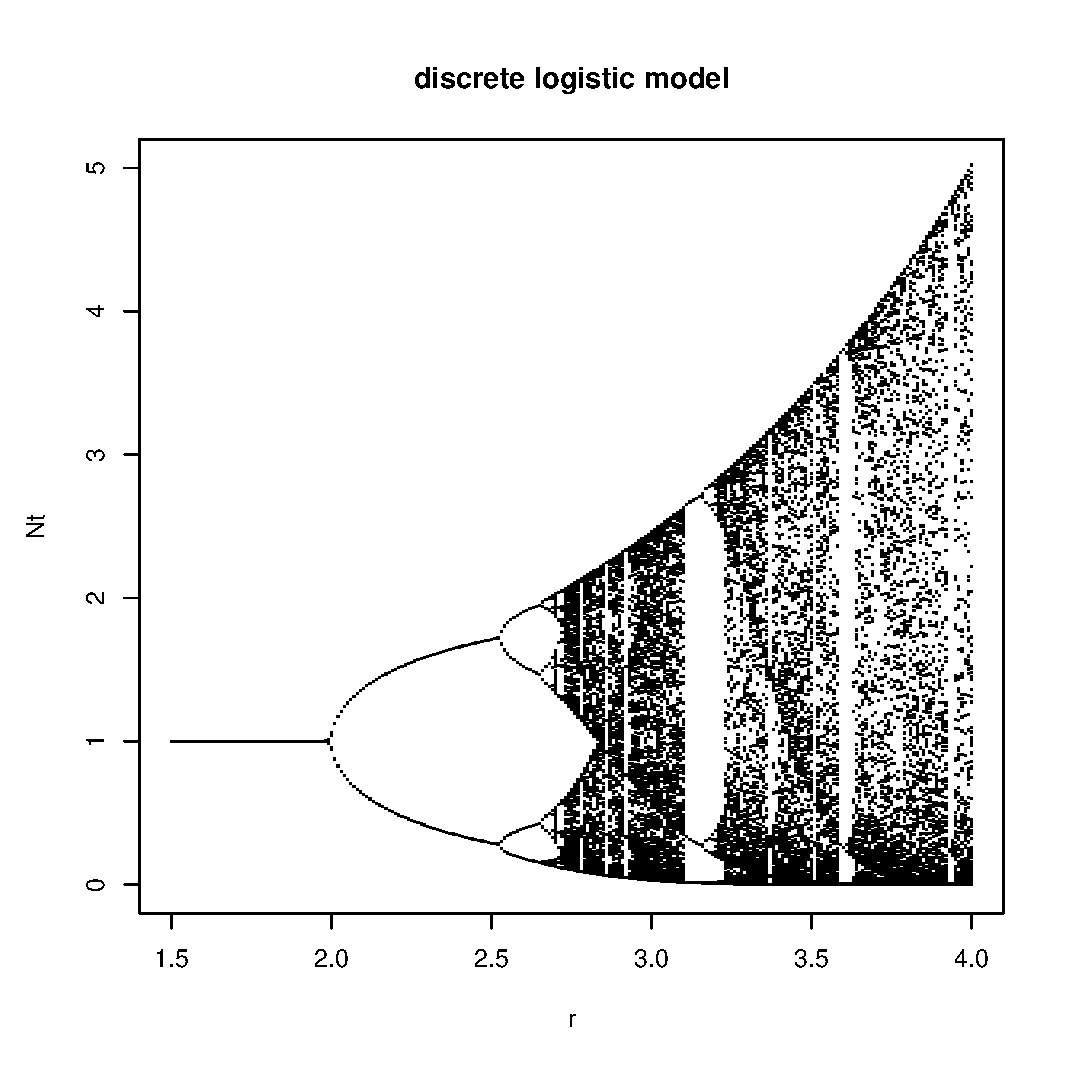
\includegraphics[height=0.75\textheight]{bifurcation_map}
		\end{center}

	\end{frame}
%------------------------------
	\begin{frame}[fragile]{The R script}
		
	\begin{lstlisting}
		ricker = function(N,r) N*exp(r*(1-N)) 
		rseq = seq(1.5,4,0.01) # sequence of r-values

		plot(0,0,xlim=range(rseq),ylim=c(0,5),type="n",
		xlab="r",ylab="Nt",main="discrete logistic model")

		for ( r in rseq)
 		{
			N = runif(1)
		 	for (i in 1:200) N = ricker(N,r)   # spinup 
			for (i in 1:200) {
				N = ricker(N,r)
				points(r,N,pch=".",cex=1.5)}
		}
		\end{lstlisting}
	\end{frame}

%------------------------------
	\begin{frame}[fragile]{Numerical approximation and numerical errors}
		\begin{center}
			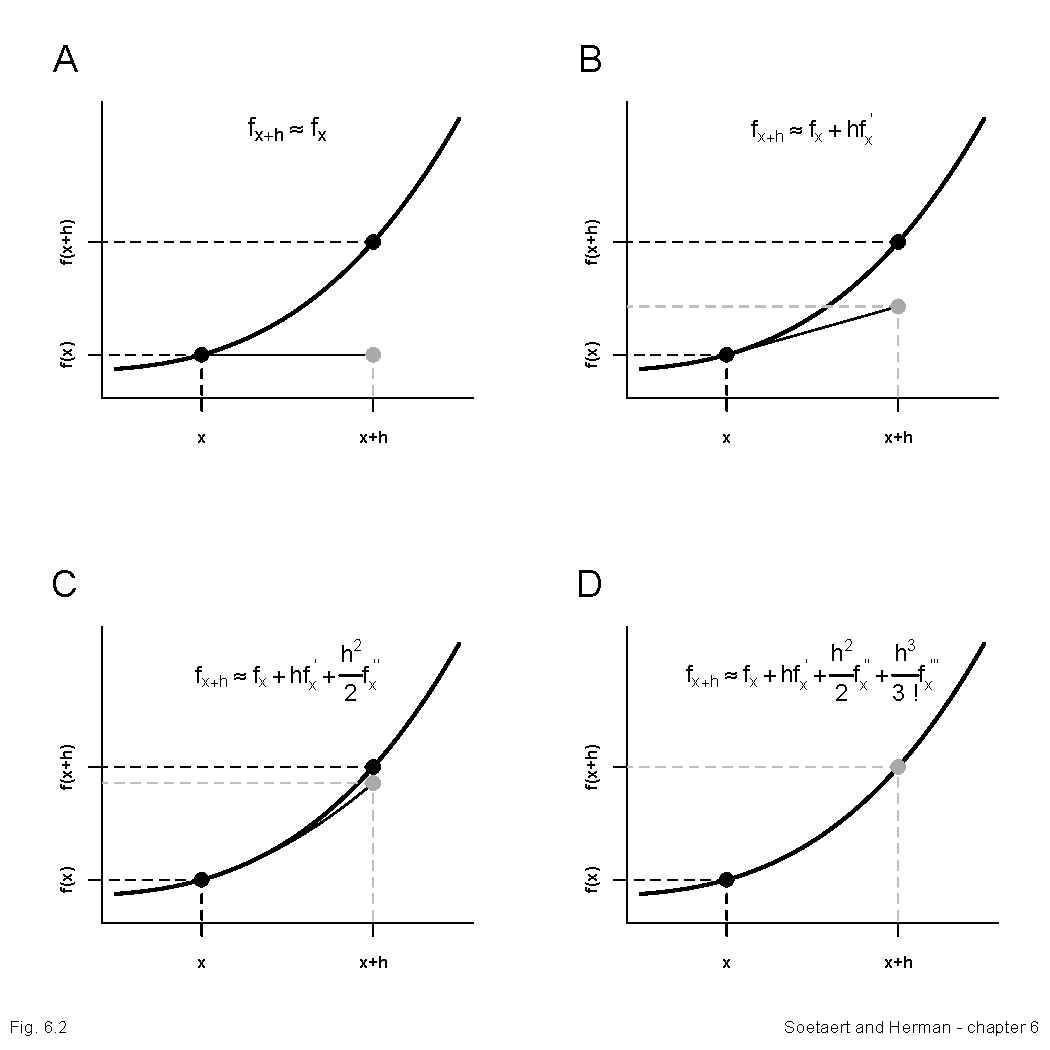
\includegraphics[height=0.75\textheight]{fig6_2}
		\end{center}
	\end{frame}

%------------------------------
	\begin{frame}[fragile]{Numerical approximation and numerical errors}
		\begin{center}
			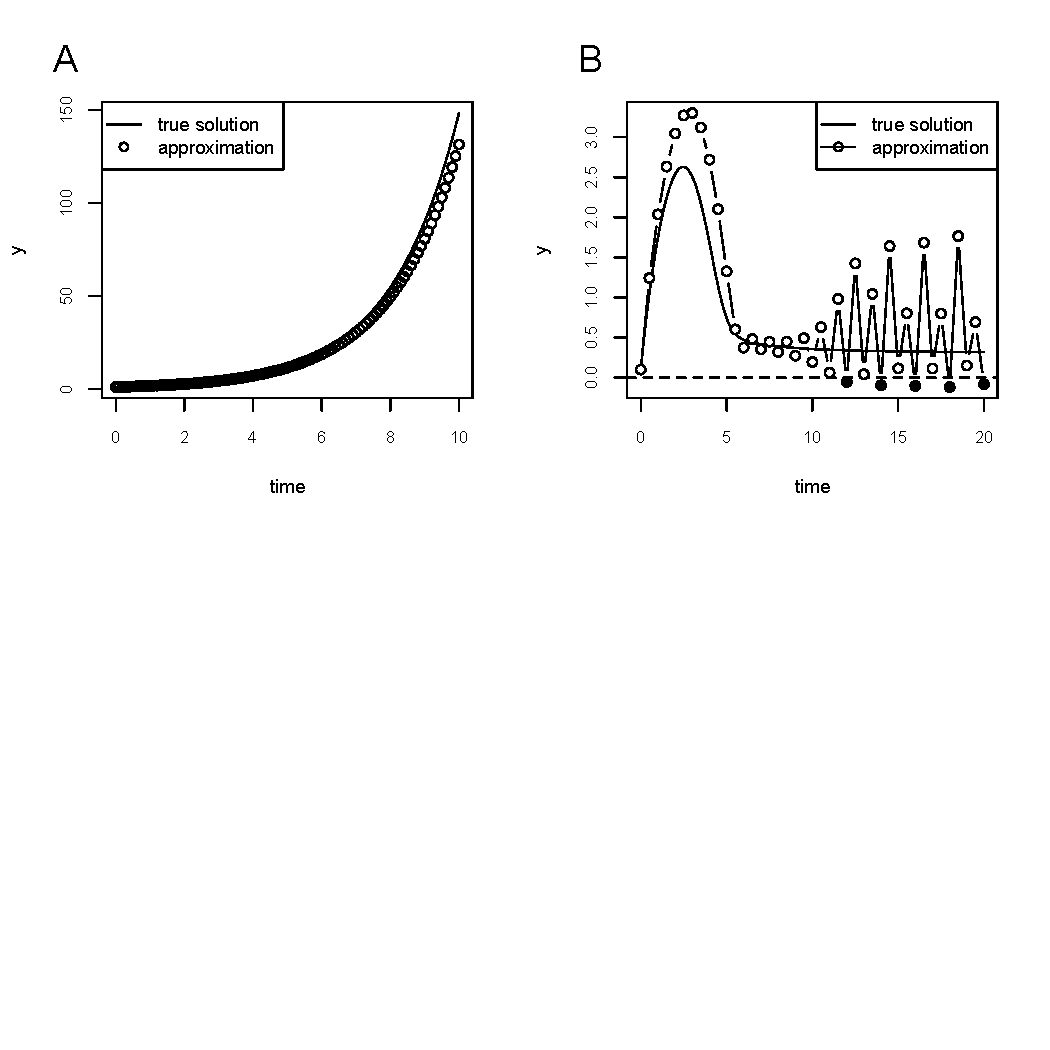
\includegraphics[height=0.55\textheight]{fig6_3}
		\end{center}
	\end{frame}

%------------------------------
	\begin{frame}[fragile]{The R script}
		
		\begin{lstlisting}
			library(ecolMod)
			demo(chap6)
		\end{lstlisting}

	\end{frame}

%------------------------------
	\begin{frame}{Criteria for numerical integration}
		
		\textbf{Accurracy} is a measure for the correctness of the solution. Relates to the approximation of the solution. Generally higher order methods are more accurante.
		\vskip 1em

		\textbf{Stability} refers to the potential of the method to lead to increasing oscillations between consecutive solution points. A consequence of the approximations. Some models are more sensitive than others.
		\vskip 1em
		
		\textbf{Speed} is the inverse of time required to compute the numerical integration. It does not matter nowadays for simple systems of differential equations, but it could be significant for large systems such as food webs or metacommunities. 
		\vskip 1em

		\textbf{Memory} increases with the complexity of the integration routine (basically the high order derivatives in the Taylor expansion

	\end{frame}

%------------------------------
	\section{Runge Kutta}

	\begin{frame}{Runge kutta integration}

	\textbf{Principle:} the method use extra evaluations of the differential equations at various positions in time and interpolate between them. The most common method is the 4th order:\\
	$N_{t+\Delta t} = N_t + \frac{h}{6}(k_1+2k_2+2k_3+k_4)$\\
	\vskip 1em

	where:\\
	$k_1 = f(t,N_t)$\\
	$k_2 = f(t+\frac{\Delta t}{2}, N_t + \frac{\Delta t}{2}k_1)$\\
	$k_3 = f(t+\frac{\Delta t}{2}, N_t + \frac{\Delta t}{2}k_2)$\\
	$k_4 = f(t+\Delta, N_t + \Delta tk_3)$\\

	\end{frame}

%------------------------------

	\begin{frame}[fragile]{Numerical approximation and numerical errors}
		\begin{center}
			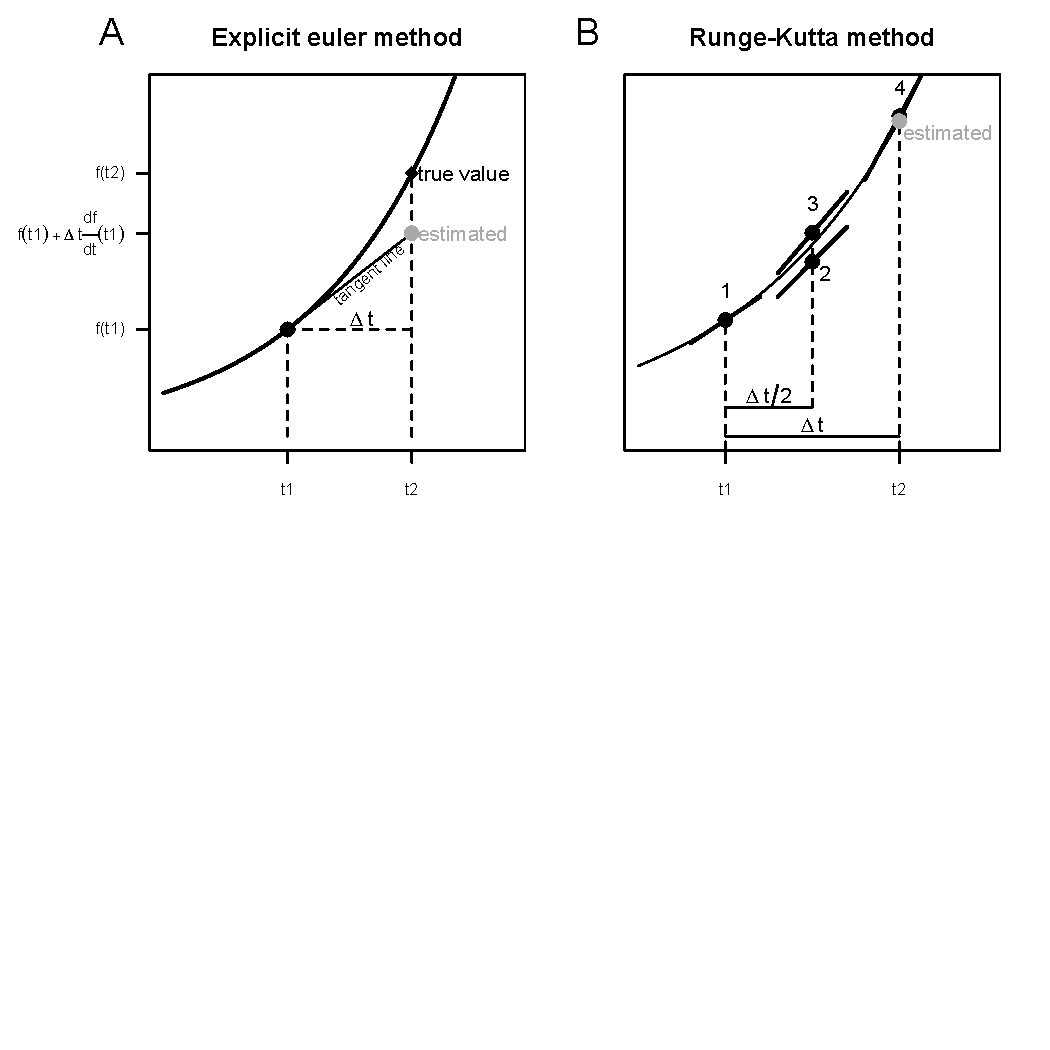
\includegraphics[height=0.55\textheight]{fig6_5}
		\end{center}
	\end{frame}

%------------------------------

	\begin{frame}[fragile]
		
		\begin{lstlisting}
			# The function to integrate
			dNdt = function(N,lambda) lambda*N

			# Calculate the amount of change:
			k1 = dNdt(N0,lambda = 1)
			k2 = dNdt(N0 + 0.5*k1)
			k3 = dNdt(N0 + 0.5*k2)
			k4 = dNdt(N0 + k3)
			delta = (k1 + 2*k2 + 2*k3 + k4)/6

			# Calculate the next density
			N1 = N0 + delta

		\end{lstlisting}

	\end{frame}

%------------------------------

	\begin{frame}{Exercise 3}
			
		Redo the steps of exercise 2, but with the Runge Kutta 4 integration method. Compare the results. Try different $\Delta t$.
	\end{frame}

%------------------------------

	\begin{frame}{Exercise 4}
			
		Compute the numerical integration of the Rosensweig-MacArthur model of predator prey interactions:\\
		$\frac{dR}{dt} = rR(1-\frac{R}{K}) - \frac{aRC}{1+bR}$\\
		$\frac{dC}{dt} = \frac{aRC}{1+bR} - dC$\\
		\vskip 1em

		Consider the parameters $r = 1, a = 1, b = 5, d = 0.1$. Try different values of $K$ within the range$[0.4,0.8]$. What happens?

	\end{frame}

%------------------------------

	\section{Libraries}

	\begin{frame}[fragile]{Librairies for ODEs}{deSolve}
		\begin{lstlisting}
		# Load the library
		library(deSolve)

		# Define the mathematical model
		model = function(Time, State, Pars) {
		with(as.list(c(State,Pars)), {
			dR = r*R*(1-R/K) - a1*R*C/(1+b*R)
			dC = a*R*C/(1+b*R) - d*C
			list(c(dR,dC))
		})
		}
		\end{lstlisting}
	\end{frame}

%------------------------------

	\begin{frame}[fragile]{Librairies for ODEs}{deSolve}
		\begin{lstlisting}
		# Define the parameters
		r = 1
		a = 1
		b = 5
		K = 0.6

		# Collect them in a vector
		pars = c(r = r, a = a, b = b, K = K)

		# Set the initial conditions
		T0 = c(R = 1, C = 0.1)

		# Set the conditions for the simulation
		times = seq(0, 1000, by = 0.1) # THE BY ARGUMENT SPECIFIES THE INTEGRATION STEP
		\end{lstlisting}
	\end{frame}

%------------------------------

	\begin{frame}[fragile]{Librairies for ODEs}{deSolve}

		\begin{lstlisting}
		# Run the simulation
		out = ode(func=model, y = T0, parms = pars, times = times)

		# Plot the results
		par(mar = c(5,6,2,1)
		plot(out[,1],out[,2],type="l",xlab = "Time",ylab = "Density",cex.lab = 1.75, 
		cex.axis = 1.5,ylim=range(out[,2:3]))  
		lines(out[,1],out[,3],col = "blue")  

		\end{lstlisting}
	\end{frame}

%------------------------------

	\begin{frame}[fragile]{rootSolve}{Compute steady state solution}
		\begin{lstlisting}
			library(rootSolve)
	
			# Specify the model
			model = function(t,y,pars) {
			with(as.list(c(y,pars)), {
				dR = r*R*(1-R/K) - a*R*C/(1+b*C)
				dC = a*R*C/(1+b*R) - d*C 		
				list(c(dR,dC))
				})
			}

			# Parameters
			pars = c(r = 1, K = 0.7, a = 1, b = 5, d = 0.1)	

			# Initial conditions
			T0 = c(R = 0.1, C = 1.1)
 	
			# Solve the model using stode (iterative state solver)
			eq = stode(y=T0, func=model, parms=pars, pos=TRUE)
		\end{lstlisting}

	\end{frame}

%------------------------------

	\begin{frame}[fragile]{rootSolve}{Jacobian matrix}
		\begin{lstlisting}
			# Compute the jacobian
			J = jacobian.full(y=eq,func=model,parms=pars)
		
			# Compute the eigen values
			eigen(J)$values
		\end{lstlisting}
	\end{frame}

%------------------------------

	\begin{frame}[fragile]{rootSolve}{Example: boundary conditions with the R-M model}

		\begin{lstlisting}
			# Vecteur of K values
			Ks = seq(0.5,1,0.01)

			# Vector to store the results
			res = numeric(length(Ks))

			# Loop to calculate eigen values for each K value
			for(i in 1:length(Ks)) {	
				pars = c(r = 1, K = Ks[i], a = 1, b = 5, d = 0.1)
				eq = stode(y=eq, func=model, parms=pars, pos=TRUE)[[1]]
				J = jacobian.full(y=eq,func=model,parms=pars)
				res[i] = max(as.real(eigen(J)$values))
			}
	
			# Plot the results
			par(mar = c(5,6,2,1),mfcol=c(1,3))
			plot(Ks,res, type = "l", xlab = "K", ylab = "Maximal eigen value", cex.axis = 1.25, cex.lab = 1.5)
			abline(h = 0, lty = 3)

			# Analytical criteria
			a = 1
			b = 5
			d = 0.1
			abline(v = (1+d*b)/(a*b*(1-d*b)), lty = 3, col = "red")
		\end{lstlisting}

	\end{frame}

%------------------------------

	\begin{frame}{Other useful functions to explore....}

		\begin{enumerate}
			\item runsteady
			\item uniroot.all
			\item multiroot
			\item steady.2D (advanced, for diffusion models)
		\end{enumerate}
	\end{frame}

%------------------------------
%------------------------------
\end{document}
